\section{\cphash{} Design}
\label{sec:design}

Figure \ref{fig:mcstore} provides a top-level view of \cphash{}'s design.
\cphash{} splits a hash table into several independent parts, which we call
\textit{partitions}. \cphash{} uses a simple hash function to assign each
possible key to a different partition. In \cphash{} all partitions are of equal
size for simplicity. If needed, partitions can be implemented to have different
sizes using more advanced memory management and data eviction algorithms (see
Section~\ref{sec:future} for a discussion of such extensions).

Each partition has a designated server thread that is responsible for all
operations on keys that belong to it. \cphash{} pin each server thread to its
core.

Applications use \cphash{} by having client threads that communicate with the
server threads and send operations using message passing (via shared
memory). Server threads return results to the client threads also using message
passing.

\begin{figure}[t]
  \centering
  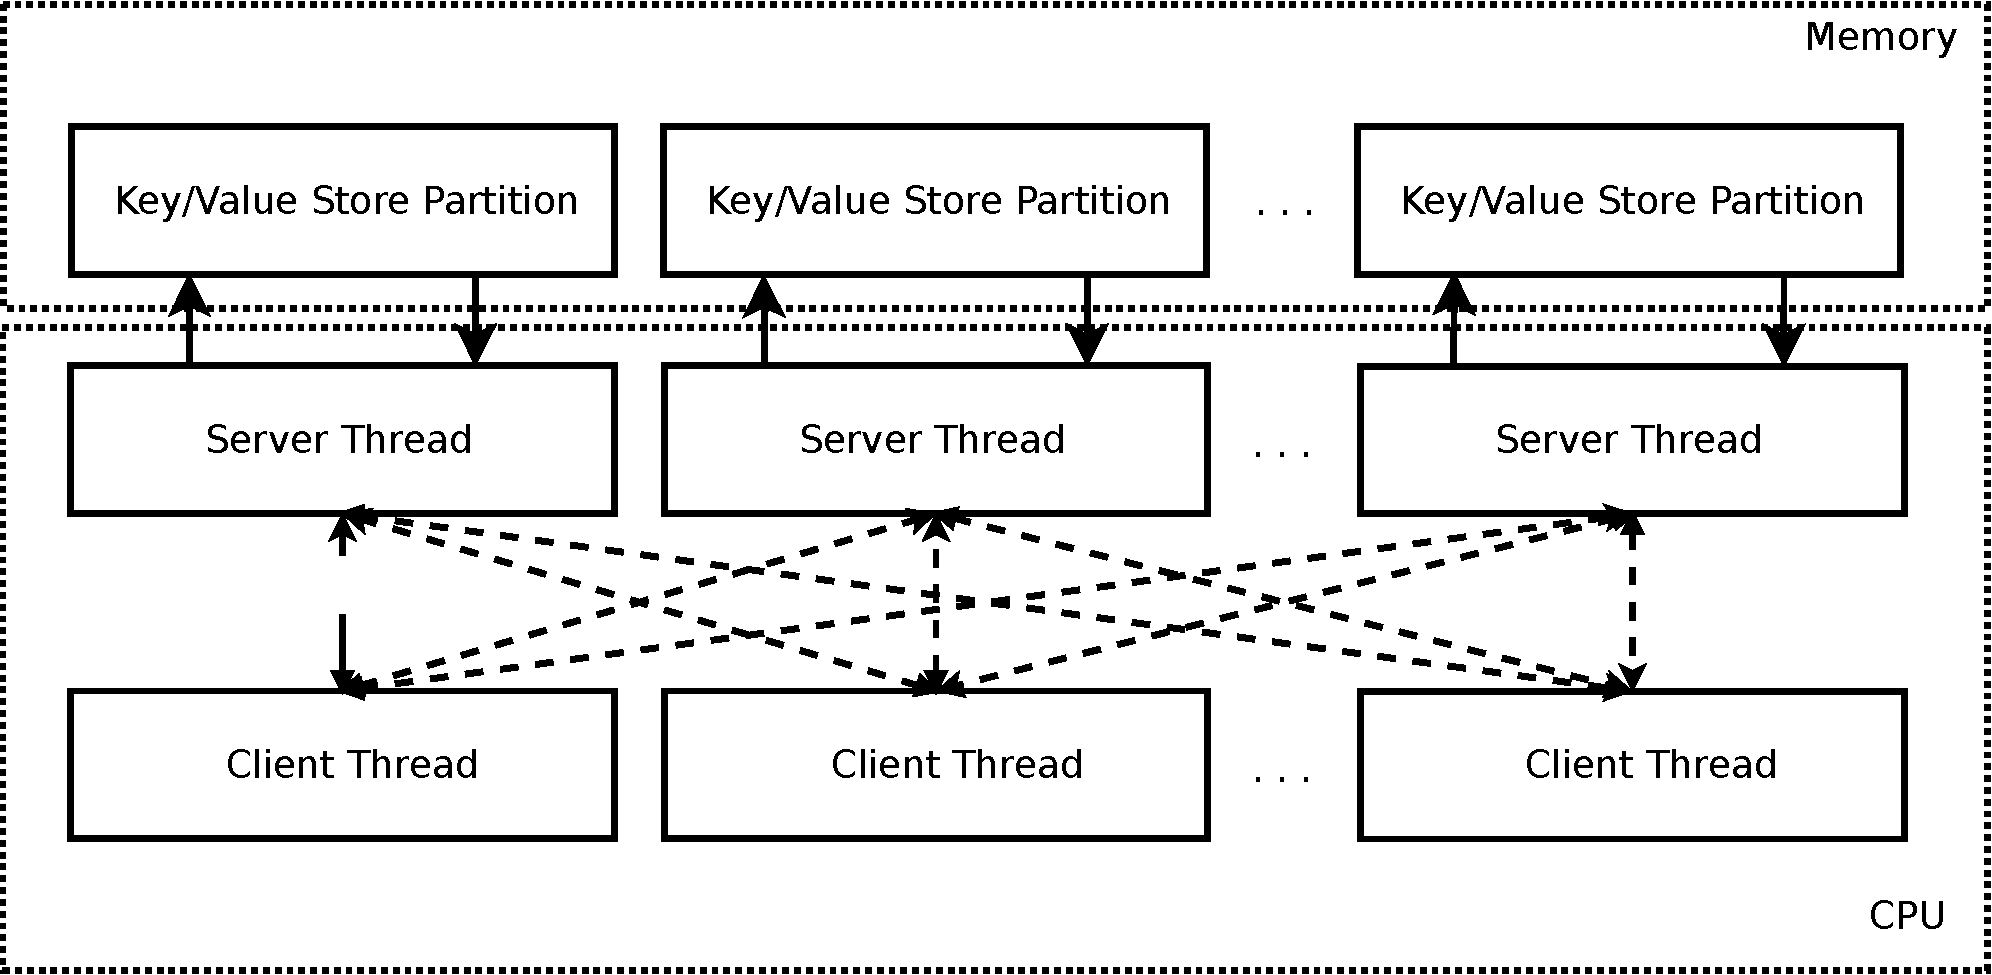
\includegraphics[width=\linewidth]{figs/mcstore.pdf}
  \caption{\cphash{} Design}
  \label{fig:mcstore}
\end{figure}

  
Section~\ref{sec:datastructure} provides a more detailed description of the
partition data structure.  Sections~\ref{sec:serverthreads}
and~\ref{sec:clientthreads} describe server and client threads, respectively..
Section~\ref{sec:msgpassing} describes the message- passing design, which
buffering and batching.  Section~\ref{sec:compmigration} discusses the benefits
of \cphash{}'s design.

\subsection{Data Structure}
\label{sec:datastructure}

Every partition in \cphash{} is a separate hash table. Figure
\ref{fig:partition} shows the partition data structure.  Each partition contains
a Bucket array. Each Bucket is a linked list. Keys are placed into different
buckets based on a hash function that maps a key to a specific bucket. Each
partition also has an LRU linked list that holds elements in the least recently
used order.  cphash{} uses LRU list to determine which elements to evict from a
partition when there is not enough space left to insert new elements.

\cphash{} pre-allocates the space that a partition can use to store data
elements at initialization.  Each element stored consists of a \texttt{key}, a
\texttt{pointer} to a value, and a \texttt{size}.  \cphash{}'s implementation
limits keys to 60-bit integer numbers; however, this can easily be extended to
support any key size (see Section \ref{sec:anykey} for more details).

\begin{figure}[t]
  \centering
  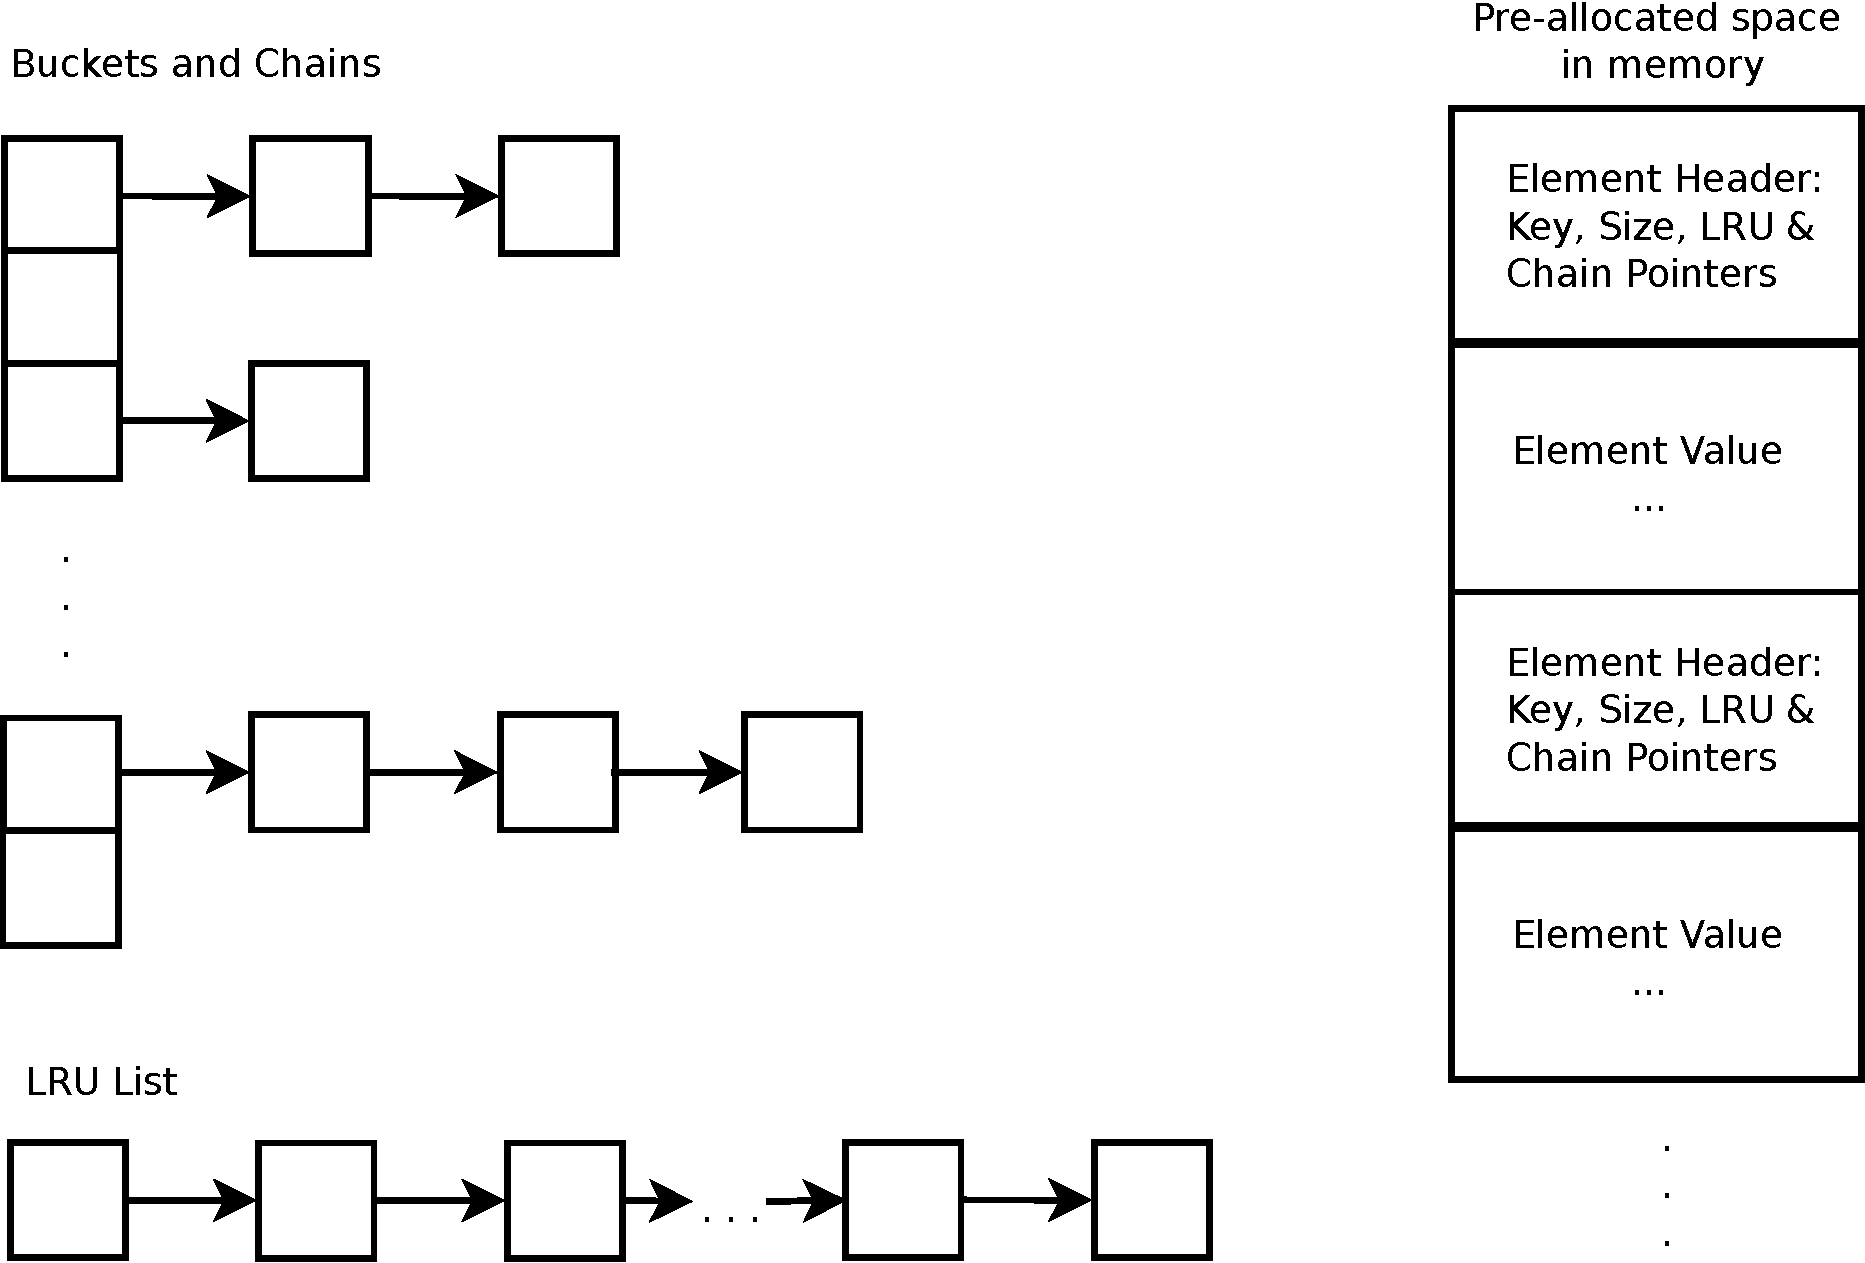
\includegraphics[width=\linewidth]{figs/partition.pdf}
  \caption{Partition Data Structure}
  \label{fig:partition}
\end{figure}

\subsection{Server Threads}
\label{sec:serverthreads}

Each server thread performs the operations for its partition.  The server thread
continuously loops over the message queues of each client checking for new
requests. When a request arrives, the server thread performs the requested
operation and sends its result back to the client.

\cphash{} supports two types of operations: \texttt{Lookup} and \texttt{Insert}.
In the case of a \texttt{Lookup}, the message contains the requested
\texttt{key}. If a key/value pair with the given \texttt{key} is found in the
partition, then the server thread updates the head of the partition's LRU list
and return the \texttt{pointer} to the value to the client thread; otherwise,
the server returns a \texttt{NULL}.

Performing an \texttt{Insert} operation is slightly more complicated. \cphash{}
is non-intrusive and supports arbitrary length values; thus, for an insert
operation memory must be allocated for the value and the value must be copied
into the allocated memory.  It is convenient to allocate memory in the server
thread since each server is responsible for a single partition and so \cphash{}
can use a standard single-threaded memory allocator.  However, performing the
actual data copying in the server thread is a bad design since for large values
it wipes out the local hardware cache of the server core. Thus, in \cphash{} the
space allocation is done in the server thread and the actual data copying is
performed in the client thread.

Thus, to perform an \texttt{Insert} operation, the server must receive the
\texttt{key} and the \texttt{size} of the data. The server thread allocates
\texttt{size} bytes of memory and removes the existing key/value pair with the
given \texttt{key} (if it exists) from the partition, to avoid having duplicate
keys for two different elements.  The allocated space is marked as ``NOT READY''
and will not be used until it is marked as ``READY''.  The client receives the
pointer, copies the data to the location pointed by the given pointer, and marks
that space as ``READY''.  The current \cphash{} implementation this marking is
done using atomic operations. 

When a server thread evicts or deletes an element from the hash table, the
memory allocated for the evicted value must be freed so that it can be reused
for new elements. It is incorrect for a server thread to just free the allocated
memory when it evicts or deletes an element. The problem is that if a client
requests a \texttt{Lookup} for some element and receives the pointer to its
value, and then the server threads evicts the element from the hash table before
the client is done processing its value, the client will have a dangling pointer
pointing to memory that might have been reallocated to a new value.  To resolve
this issue, \cphash{} counts references to an element.  Each element in the hash
table has a reference count. Every time a client requests a \texttt{Lookup} of
an element, the server thread increases the element's reference count. When the
client is done with the item, it decreases the reference count of the element.
When the reference count reaches 0, the space can be safely deallocated.
\cphash{} implements reference counting using atomic operations.

The actual deallocation must be done by a server thread, otherwise there would
be a race between allocations and deallocations within partition. When a client
decreases a reference count and it becomes zero, \cphash{} needs some way to
schedule an element for freeing in the corresponding server thread.  To do so,
\cphash{} uses a lock-free singly-linked list using atomic operations that holds
the list of elements that can be safely freed. Scheduled elements are freed in
the server thread before the next allocation.

\XXX{maybe messages are used instead of atomic instructions.}

\subsection{Client Threads}
\label{sec:clientthreads}

Applications have client threads that communicate with the server threads to
perform operations. An example of a client thread in an application is the
client thread in \cpserver{}'s implementation. The client threads in \cpserver{}
gather operations from TCP connections, route them to the appropriate server
threads, gather the results, and send them back to the correct TCP
connections. Section \ref{sec:server} describes \cpserver{}'s implementation in
more detail.  Client threads do not necessarily have to be pinned to a specific
core but, to achieve the highest performance in message passing, it is best to
keep the client threads attached to a specific core.

\subsection{Buffering and Batching}
\label{sec:msgpassing}

\cphash{} implements message passing between the client and server threads using
pre-allocated circular buffers in shared memory.  For each server and client
pair there are two arrays of buffers---one for each direction of
communication. Another possible way to implement message passing is to use a
single buffer per client/server pair, which our original design did.  Figure
\ref{fig:mpdesign} gives graphical representation for both designs.

In the single buffer implementation, space is allocated for each client/server
pair and when a client want to send a request to a server, it writes the message
to the buffer and waits for the server to respond. When the server is done
processing the message, it updates the shared location with the result.

The implementation of an array of buffers consists of the following: a data
buffer array, a read index, a write index, and a temporary write index. When the
producer wants to add data to the buffer, it first makes sure that the read
index is large enough compared to the temporary write index so that no unread
data will be overwritten. Then it writes data to buffer and updates temporary
write index. When the temporary write index is sufficiently larger than the
write index, the producer flushes the buffer by changing the write index to the
temporary write index.

To read data, the consumer waits until the read index is less than the write
index, then it proceeds to read data and update the read index. The Read Index,
write index and temporary write Index are carefully aligned in memory to avoid
any false sharing.  To decrease the number of cache misses when reading or
writing buffers, the client threads flush the buffer when the whole cache line
is full and the server threads update the read index after they are done reading
all the operations in a cache line.

\begin{figure}[t]
  \centering
  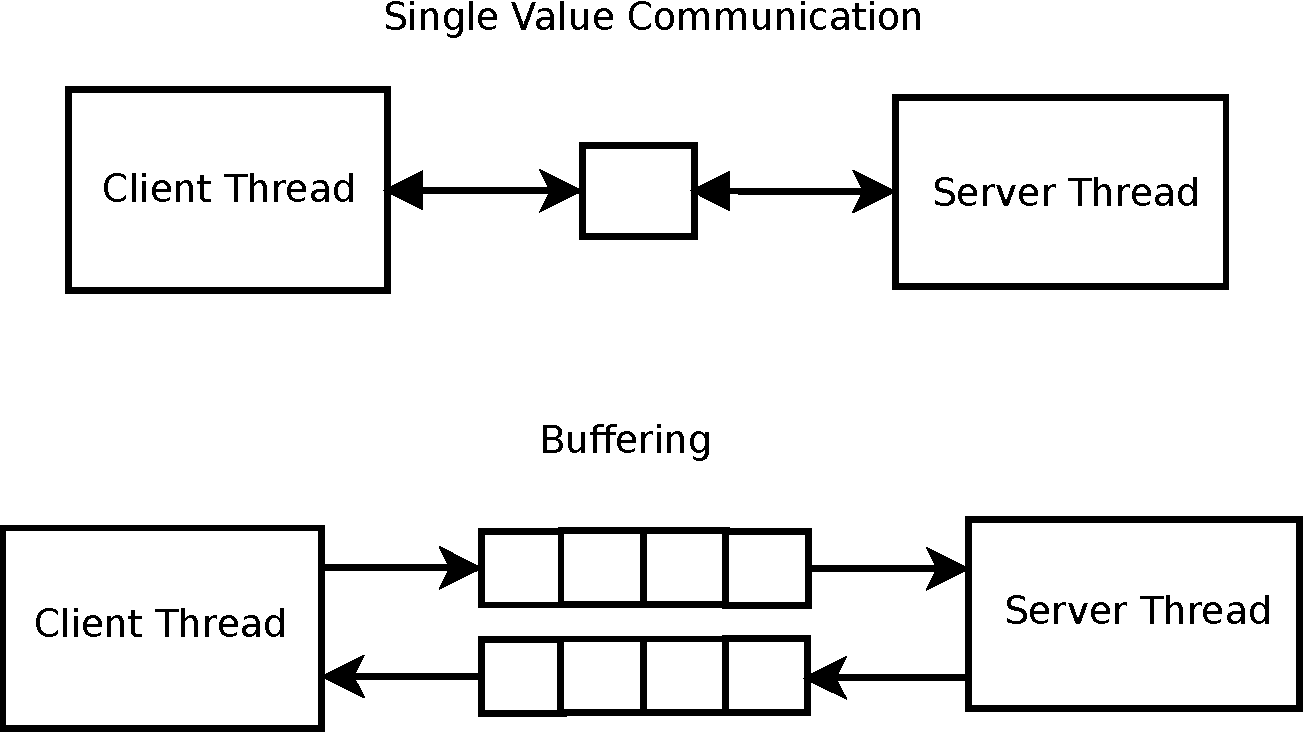
\includegraphics[width=\linewidth]{figs/mpdesign.pdf}
  \caption{Message Passing Designs}
  \label{fig:mpdesign}
\end{figure}

There are two major benefits to using arrays of buffers instead of single
buffers. The first advantage is improved parallelism.  With an array of buffers,
the client can just queue the requests to the servers; thus, even if the server
is busy, the client can continue working and schedule operations for other
servers. This way all the servers can stay busy 100\% of the time, allowing
applications to achieve better performance.

The second reason is decreased overhead for message passing.  With a single
buffer, for every message received, the server experiences a cache miss;
however, since a cache line can hold several messages (in our test machines a
cache line is 64 bytes), with buffering the server can receive several messages
using only a singe cache miss.

There are some downsides to using arrays of buffers instead of the single
buffers.  The array implementation requires having extra indices to enable the
server and the client to know how much data has been written and how much has
been read. Maintaining these indices introduces extra performance overhead that
a single buffer does not have. Thus, if the client sends requests to the server
at a slow rate, a single buffer outperforms the array implementation. However,
if the client has a batch of requests that it needs to complete, buffering will
be an advantage. Our target applications are bottlenecked by the performance of
the hash table, and have no shortage of requests; therefore, buffering is a
better design choice for message passing.

\subsection{Discussion}
\label{sec:compmigration}

There are several advantages to using messages in \cphash{}. The first advantage
is better cache performance because each partition is only modified and accessed
by a single server thread, i.e. a single core.  Since there is only one core
accessing and modifying the data, the hardware cache-coherence protocol will not
send invalidations for data that is written. Furthermore, all frequently
accessed structures, such as, the LRU list, buckets array, free list, etc can
stay in the local cache and can be read and modified fast.  Section
\ref{sec:eval} shows that this benefit results in a significant performance
improvement.

The second advantage is avoiding synchronization for shared data access. Since
each partition is modified by only one core, there is no need for any
synchronization mechanisms to protect the data from races. In addition to
performance benefits, this approach also provides the benefit of ease of
implementation.  The operations on the data structure operations don't have to
multithreaded and, thus, no changes are necessary from the single threaded
implementation.

The more difficult part of the \cphash{} implementation is message passing;
however, the message passing design and implementation can be standardized and
the message passing design and implementation can stay exactly the same for many
other data structures.

